\documentclass[conference]{IEEEtran}
\renewcommand{\abstractname}{Resumen}
\renewcommand{\IEEEkeywordsname}{Palabras clave}
\renewcommand{\refname}{REFERENCIAS}
\IEEEoverridecommandlockouts
% The preceding line is only needed to identify funding in the first footnote. If that is unneeded, please comment it out.
\usepackage{cite}
\usepackage{amsmath,amssymb,amsfonts}
\usepackage{algorithmic}
\usepackage{graphicx}
\usepackage{textcomp}
\usepackage{xcolor}
\def\BibTeX{{\rm B\kern-.05em{\sc i\kern-.025em b}\kern-.08em
    T\kern-.1667em\lower.7ex\hbox{E}\kern-.125emX}}

\begin{document}

\title{Proyecto integrador de Arquitectura y Ensamblador}

\author{\IEEEauthorblockN{Emanuel Hernández Arauz}
\IEEEauthorblockA{\textit{E.C.C.I} \\
\textit{Universidad de Costa Rica}\\
San José, Costa Rica \\
emanuel.hernandezarauz@ucr.ac.cr}
\and
\IEEEauthorblockN{Erlien Foulkes Barrantes}
\IEEEauthorblockA{\textit{E.C.C.I} \\
\textit{Universidad de Costa Rica}\\
San José, Costa Rica \\
erlien.foulkes@ucr.ac.cr}
}

\maketitle

\begin{abstract}
El presente documento contiene una descripción detallada de la primera fase del proyecto integrador de arquitectura y ensamblador,
el cual consiste en modelar el juego de mesa reversi, utilizando estructuras de datos de un máximo de $R^2$ dimensiones haciendo uso del lenguaje ensamblador,
esto con el fin de lograr una mayor eficiencia al momento de la ejecución del programa, aprovechando las prestaciones y beneficios que brinda el uso de este lenguaje.
\end{abstract}

\begin{IEEEkeywords}
lenguaje ensamblador, reversi, othelo, juegos de mesa, estructuras de datos, arreglos, manejo de memoria.
\end{IEEEkeywords}

\section{Introducción}

La finalidad de este proyecto es entender y utilizar el lenguaje de programación "ensamblador" para realizar un videojuego llamado "reversi".
El desarrollo del mismo iniciara por una propuesta de diseño que será realizada en un formato modular el cual facilitará el dividir el proyecto a programar en varias partes más sencillas las cuales funcionarán en conjunto dando para funcionar como un juego.

\section{Desarrollo}
\subsection{Descripción del juego de mesa Reversi (othelo/yang)}

El juego consta de un tablero de 8 filas por 8 columnas (64 casillas) similar al del ajedrez, 
en el que se colocan fichas redondas que constan de una cara negra y una cara blanca.

Reglas:



\subsection{Descripción y funcionamiento de los módulos}

\begin{itemize}
    \item Tablero: se entiende como tablero a una tabla cuadriculada en la cual cada cuadrícula (también llamada casilla) tiene la posibilidad de estar vacía o puede tener una ficha ya sea blanca o negra
    \item Ficha: Representación del como se encuentra la casilla (vacía, ficha blanca o negra)
    \item Vaciar: convierte la casilla en una ficha blanca
    \item Colocar:ncoloca una ficha en una zona del tablero
    \item Ver: representación de como se encuentra el tablero
    \item Estado:
    \item Verificar estado partida:
    \item Jugador:
    \item Alternar Jugador:
    \item Calcular puntos:
    \item Movida:
    \item Validar jugada:
    \item Flanquear:
\end{itemize}

\section{Resultados Esperados}
Se espera conseguir un diseño funcional del juego de mesa llamado "reversi" a través del uso de lenguaje ensamblador y a su vez implementar una interfaz gráfica utilizando "C"


\end{document}







% Comandos frecuentes by EMA
\subsection{Subtítulo}

\section{Seccón con ref.}
\ref{AAREF}

\subsection{Subtítulo con ref.}\label{AAREF}

\begin{equation}
a+b=\gamma\label{eq}
\end{equation}

\begin{itemize}
\item it1
\item it2
\end{itemize}

\paragraph{Parrafo} Place figures and tables at the top and 
bottom of columns.
``Fig.~\ref{fig}'', even at the beginning of a sentence.

\begin{table}[htbp]
\caption{Table Type Styles}
\begin{center}
\begin{tabular}{|c|c|c|c|}
\hline
\textbf{Table}&\multicolumn{3}{|c|}{\textbf{Table Column Head}} \\
\cline{2-4} 
\textbf{Head} & \textbf{\textit{Table column subhead}}& \textbf{\textit{Subhead}}& \textbf{\textit{Subhead}} \\
\hline
copy& More table copy$^{\mathrm{a}}$& &  \\
\hline
\multicolumn{4}{l}{$^{\mathrm{a}}$Sample of a Table footnote.}
\end{tabular}
\label{tab1}
\end{center}
\end{table}

\begin{figure}[htbp]
\centerline{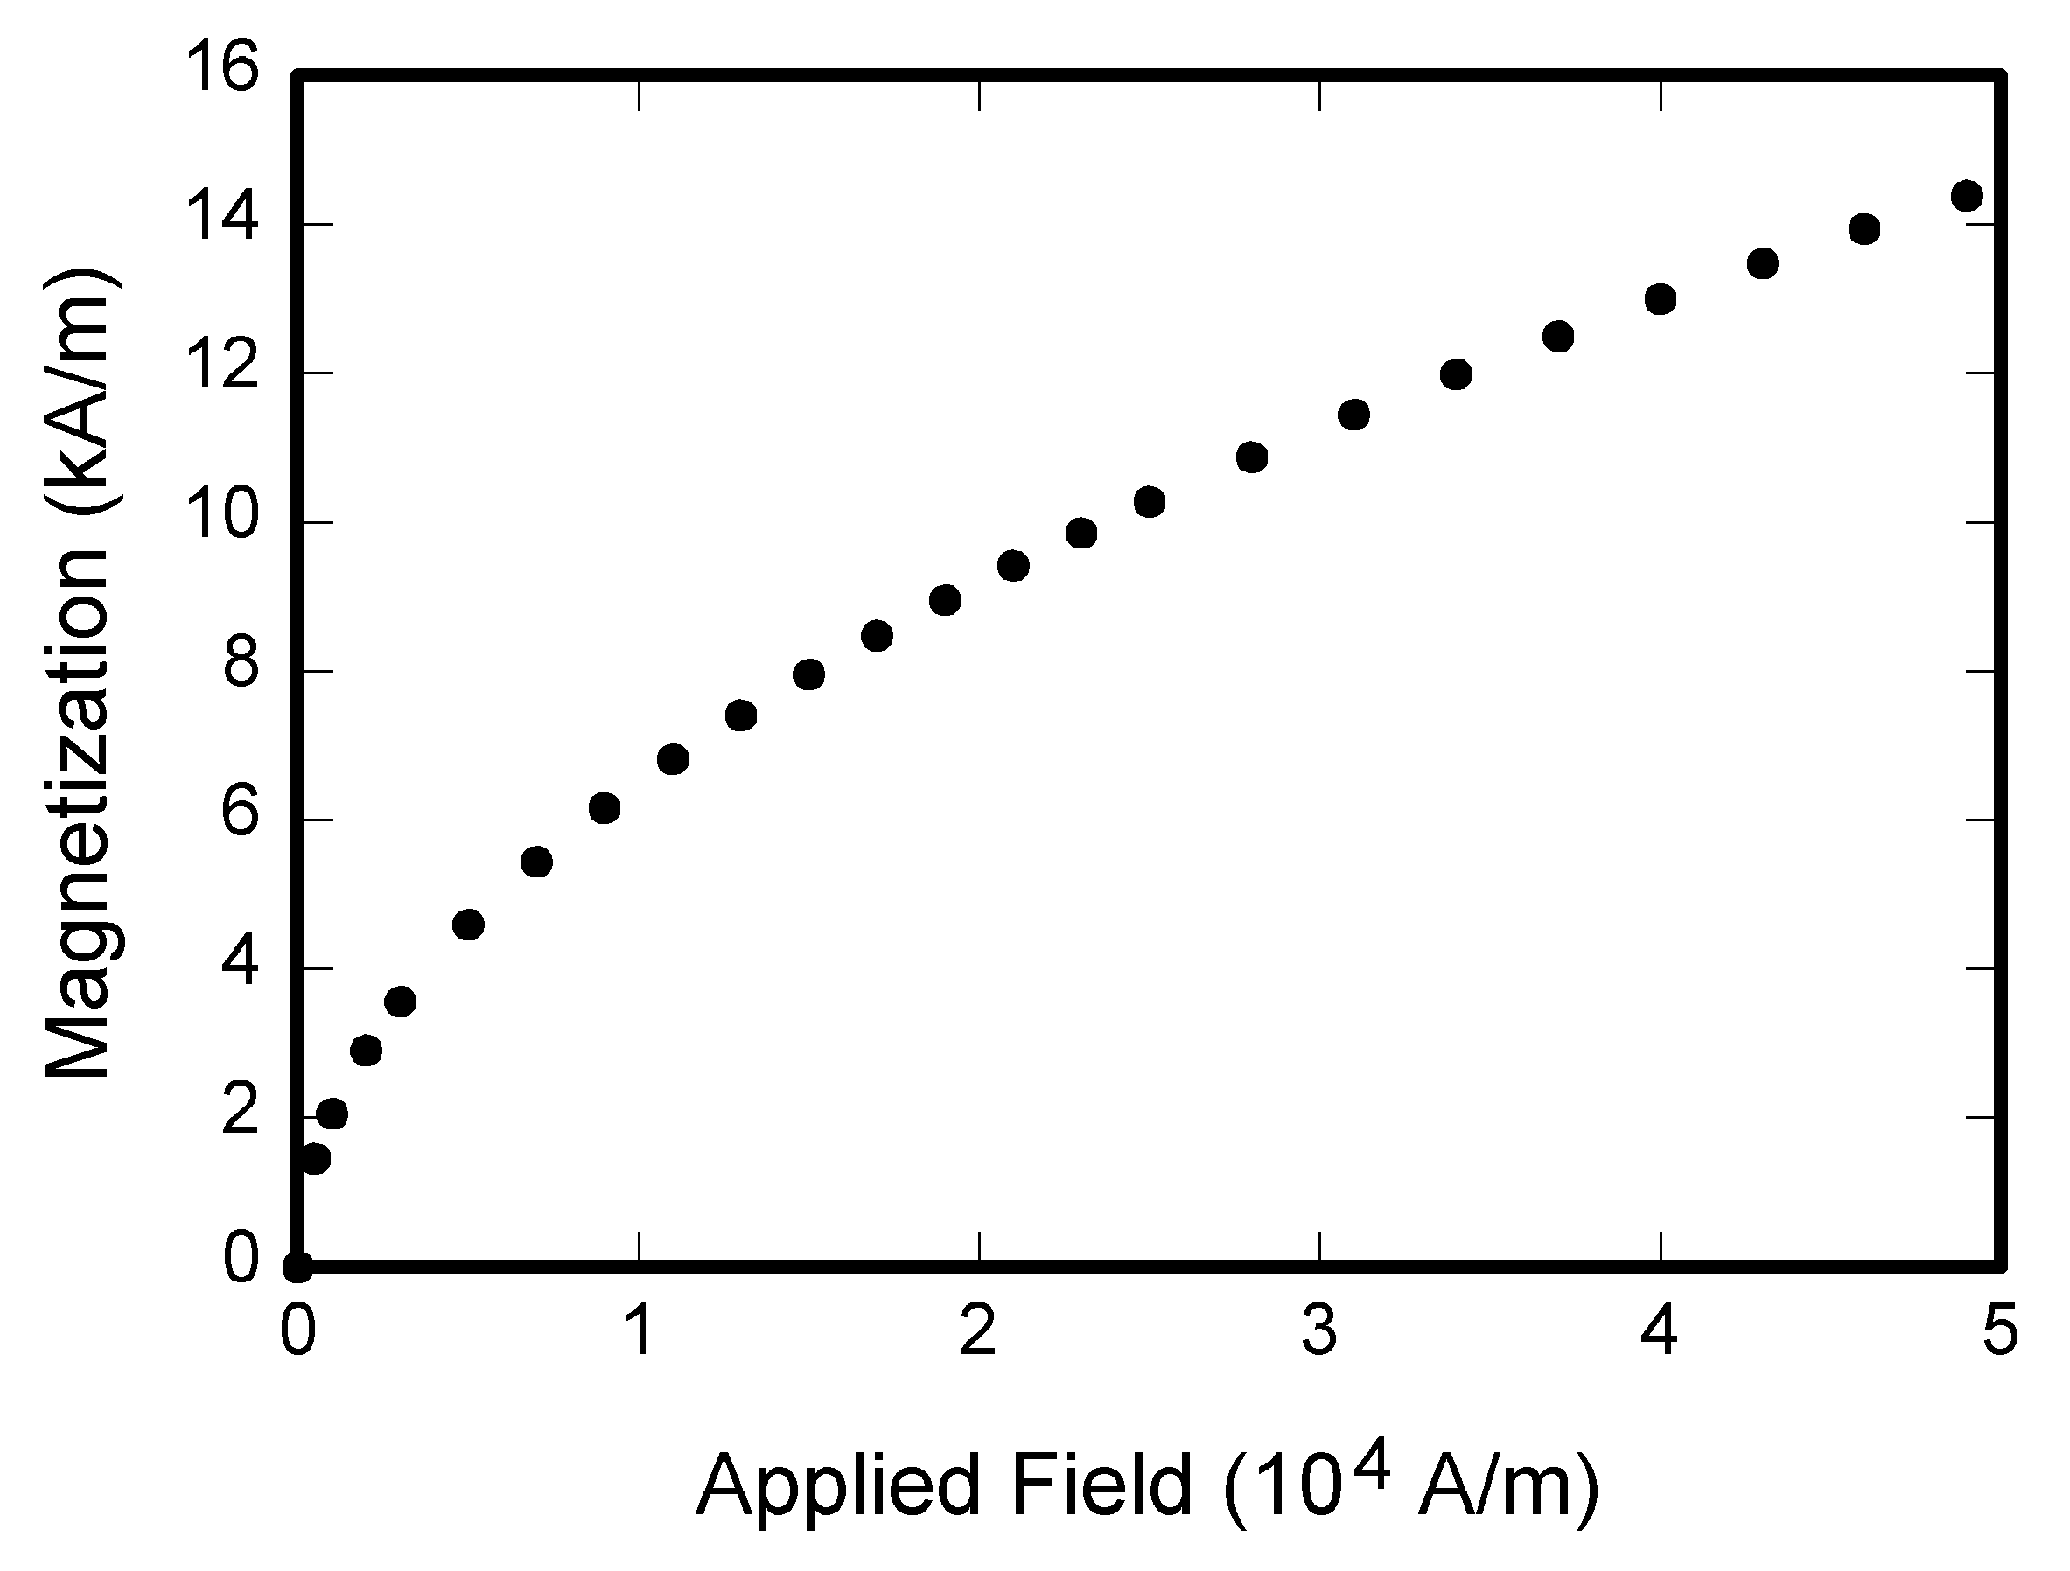
\includegraphics{fig1.png}}
\caption{Ejemplo de figura}
\label{fig}
\end{figure}

\cite{b1}. 

\begin{thebibliography}{00}
\bibitem{b1} G. Eason, B. Noble, and I. N. Sneddon, ``On certain integrals of Lipschitz-Hankel type involving products of Bessel functions,'' Phil. Trans. Roy. Soc. London, vol. A247, pp. 529--551, April 1955.
\end{thebibliography}